%% ----------------------------------------------------------------------
%%
%% apa7 - A LaTeX class for formatting documents in compliance with the
%% American Psychological Association's Publication Manual, 7th edition
%%
%% Copyright (C) 2019 by Daniel A. Weiss <daniel.weiss.led at gmail.com>
%%
%% This work may be distributed and/or modified under the
%% conditions of the LaTeX Project Public License (LPPL), either
%% version 1.3c of this license or (at your option) any later
%% version.  The latest version of this license is in the file:
%%
%% http://www.latex-project.org/lppl.txt
%%
%% Users may freely modify these files without permission, as long as the
%% copyright line and this statement are maintained intact.
%%
%% This work is not endorsed by, affiliated with, or probably even known
%% by, the American Psychological Association.
%%
%% ----------------------------------------------------------------------

\documentclass[man,floatsintext,hidelinks]{apa7}

\usepackage{lipsum}
\usepackage{listings}
\usepackage{xcolor}
\usepackage{hyperref}
\urlstyle{same}

\usepackage{pdflscape}
\usepackage[american]{babel}
\usepackage{graphicx}
\usepackage{longtable} 
\usepackage{array}
\usepackage{setspace}
\usepackage{lineno}
\pagewiselinenumbers
\raggedbottom

%\usepackage{titlesec}
%\titlespacing*{\section}{0pt}{0ex}{0ex}
%\titlespacing{\subsection}{0pt}{0ex}{-1ex}
%\titlespacing*{\subsubsection}{0pt}{0ex}{-2ex}

\setlength{\parskip}{1em plus0mm minus0mm}

\usepackage{csquotes}
\usepackage[style=apa,sortcites=true,sorting=nyt,backend=biber]{biblatex}
\DeclareLanguageMapping{american}{american-apa}
\addbibresource{refs.bib}

\title{Meta-analytic findings of the self-controlled motor learning literature: Underpowered, biased, and lacking evidential value}
\shorttitle{Meta-analysis of self-controlled research}

\author{Brad McKay\textsuperscript{1}, Zachary D. Yantha\textsuperscript{1}, Julia Hussien\textsuperscript{1}, Michael J. Carter\textsuperscript{2}, and Diane M. Ste-Marie\textsuperscript{1}}


\affiliation{\vspace*{18pt}\textsuperscript{1}\emph{School of Human Kinetics, University of Ottawa} \\
			 \textsuperscript{2}\emph{Department of Kinesiology, McMaster University}}

\leftheader{}

\abstract{The self-controlled motor learning literature consists of experiments that compare a group of learners who are provided with a choice over an aspect of their practice environment to a group who are yoked to those choices. A qualitative review of the literature suggests an unambiguous benefit from self-controlled practice. A meta-analysis was conducted on the effects of self-controlled practice on retention test performance measures with a focus on assessing and potentially correcting for selection bias in the literature, such as publication bias and \emph{p}-hacking. First, a naïve random effects model was fit to the data and a moderate benefit of self-controlled practice, $g = .44\,(k = 52, N = 3134, 95\%\,CI\,[.31,\,.56])$, was found. Second, publication status was added to the model as a potential moderator, revealing a significant difference between published and unpublished findings, with only the former reporting a benefit of self-controlled practice. Third, to investigate and adjust for the impact of selectively reporting statistically significant results, a weight-function model was fit to the data with a one-tailed \emph{p}-value cutpoint of .025. The weight-function model revealed substantial selection bias and estimated the true average effect of self-controlled practice as $g = .107\,(95\%\,CI\,[.047,\,.18])$. \emph{P}-curve analyses were conducted on the statistically significant results published in the literature and the outcome suggested a lack of evidential value. Fourth, a suite of sensitivity analyses were conducted to evaluate the robustness of these results, all of which converged on trivially small effect estimates. Overall, our results suggest the benefit of self-controlled practice on motor learning is small and not currently distinguishable from zero.
}

\keywords{Motor learning, retention, choice, ``OPTIMAL'' theory, meta-analysis, \emph{p}-curve, publication bias}

\authornote{
  \addORCIDlink{Brad McKay}{0000-0002-7408-2323}
  
  \addORCIDlink{Zachary D. Yantha}{0000-0003-1851-7609}
  
  \addORCIDlink{Julia Hussien}{0000-0001-7434-228X}
  
  \addORCIDlink{Michael J. Carter}{0000-0002-0675-4271}
  
  \addORCIDlink{Diane M. Ste-Marie}{0000-0002-4574-9539}

Correspondence concerning this article should be addressed to Brad McKay. E-mail: \href{mailto:bradmckay8@gmail.com}{bradmckay8@gmail.com}
}

\begin{document}

\maketitle

Asking learners to control any aspect of their practice environment has come to be known as self-controlled practice in the motor learning literature \parencite{Sanli2013-xn,Wulf2016-gf}. The first published experiments to test self-controlled learning asked learners to control their augmented feedback schedule \parencite{Janelle1995-rj,Janelle1997-ht}. For example, in an experiment by \Textcite{Janelle1997-ht}, participants practiced throwing tennis balls at a target with their non-dominant hand. The practice period occurred over two separate days. Participants were assigned to one of four experimental groups (\emph{n} = 12): Self-controlled knowledge of performance (KP), yoked-to-self-control, summary KP after every 5 trials, and a knowledge of results only control group. The self-controlled group could request KP whenever they wanted it, while each yoked group participant was matched with a self-control group counterpart and received KP on the same schedule. The experimenter evaluated the participants’ throws, identified the most critical error in their throwing form, and provided KP via video feedback, along with directing attention to the error and giving prescriptive feedback. During a delayed-retention test, the accuracy, form, and speed of the throw were assessed. The results indicated that the self-control group threw more accurately and with better form than all other groups on the retention test. The self-control and yoked groups did not significantly differ in throwing speed, but the control group threw faster than the self-control group on the second retention block. The results were interpreted as evidence that the participants provided with choice were able to process information more efficiently than their counterparts who received a fixed schedule of feedback.

\begin{figure}[h]
	\caption{Number of self-controlled learning experiments meeting the inclusion criteria by year.}
	\centering
    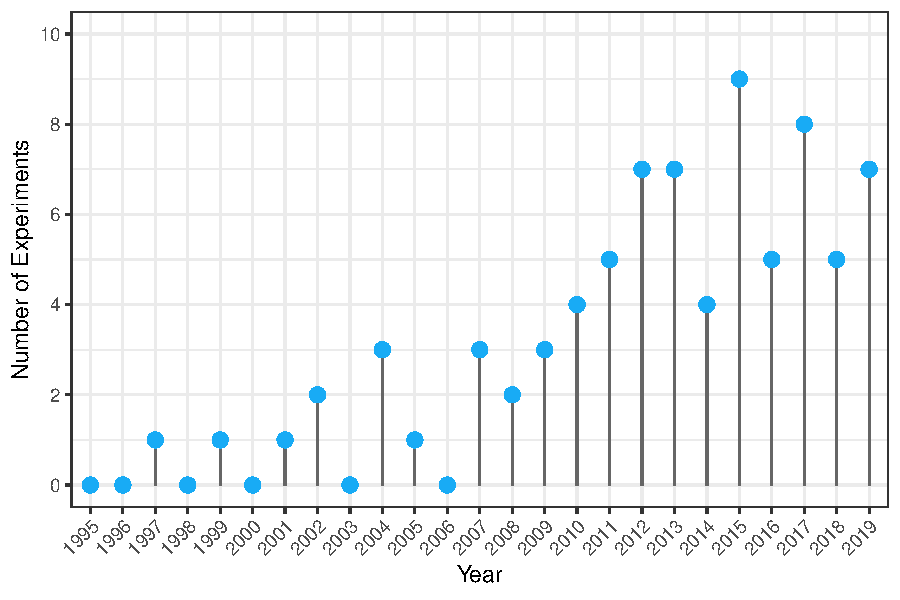
\includegraphics[]{figs/fig1.pdf}
    \label{fig:Figure1}
\end{figure}

Figure~\ref{fig:Figure1} shows that the number of experiments comparing self-controlled groups to yoked groups has been increasing since the original experiments by Janelle and his colleagues (1995; 1997). Researchers have experimented with giving learners control over a variety of variables in the practice environment. A qualitative assessment of the literature suggests that self-control is generally beneficial regardless of choice-type \parencite{Wulf2016-gf}. For example, self-control has been effective when participants have been provided choice over what can be considered instructionally-relevant variables, such as: knowledge of results (KR) \parencite{Patterson2010-tk}, KP \parencite{Lim2015-qs}, concurrent feedback \parencite{Huet2009-wu}, use of an assistive device \parencite{Wulf2001-nb}, observation of a skilled model \parencite{Lemos2017-qx}, practice schedule \parencite{Wu2011-ha}, practice volume \parencite{Lessa2015-eq}, and task difficulty \parencite{Leiker2016-zd}. Additionally, self-controlled benefits have also been found for instructionally-irrelevant variables, such as: the colour of various objects in the practice environment \parencite{Wulf2018-ie}, other decorative choices \parencite{Iwatsuki2019-tf}, and the choice of what to do after the retention test is complete \parencite{Lewthwaite2015-bd}.

Despite the widespread optimism that self-controlled practice is useful for enhancing motor learning, researchers continue to debate the underlying mechanisms responsible for the effect \parencite{Carter2017-mk,Wulf2018-ie}. Beginning with \Textcite{Janelle1995-rj}, both motivational and information processing mechanisms were proposed as possible explanations for self-control benefits. Researchers have since supported these two mechanisms and, from a motivational perspective, have posited that self-control enhances confidence \parencite{Janelle1995-rj,Chiviacowsky2012-cw,Wulf2016-gf} and satisfies the basic psychological need for autonomy \parencite{Sanli2013-xn,Wulf2016-gf}, motivating motor performance and learning enhancement. Most self-controlled learning experiments, however, have involved participants making choices over potentially informative variables, which could act as a confounding variable. Citing this potential motivational/informational confound, \Textcite{Lewthwaite2015-bd} experimented with providing instructionally-irrelevant choices, such as the colour of the golf balls to putt, the painting to hang on the wall, and what to do following the retention test. Lewthwaite and her colleagues reasoned that information processing explanations could not account for benefits due to these incidental choices, and instead motivational factors would be more likely. Consistent with the motivational hypothesis, participants exhibited significantly greater motor learning on a golf putting task (Experiment 1) and on a balance task (Experiment 2). Subsequently, several experiments have reported benefits with instructionally-irrelevant choices \parencite{Abdollahipour2017-dr,Chua2018-sn,Halperin2017-az,Iwatsuki2019-tf,Wulf2014-sn,Wulf2018-ie}, further reinforcing this motivational perspective.

A contrasting line of research has been reported by Carter and his colleagues \parencite{Carter2014-up,Carter2017-ix,Carter2017-mk} in which informational factors, the second dominant perspective, are given more weight as an explanatory variable. In one experiment \parencite{Carter2014-up}, self-control participants were provided with choice over receiving KR, but divided into three experimental groups; those who could make their KR decision: before the trial, after the trial, or both (they would decide before, but could change their mind following the trial). Timing of the choice significantly attenuated the self-control benefit. While the self-after and self-both groups exhibited learning advantages relative to their yoked counterparts, the self-before group displayed no such advantage. The argument proffered by the researchers was that there was more informational value to be gained from KR requested after a trial than when it had to be requested before the outcome of the trial occurred \parencite[also see][]{Chiviacowsky2005-iq}. 

In another experiment \parencite{Carter2017-ix}, asking learners to complete an interpolated activity in the interval preceding their choice of whether to receive KR significantly attenuated the self-control benefit \parencite[also see][]{Couvillion2020-zw,Woodard2020-uq}. As a final example, \Textcite{Carter2017-mk} compared an instructionally-relevant choice group (i.e., when to receive KR) to an instructionally-irrelevant choice group (i.e., which video game to play after retention and which colour arm wrap to wear while practicing). Unlike the experiment by Wulf and colleagues (\citeyear{Wulf2018-ie}), Carter and Ste-Marie found that instructionally-relevant choices were more effective than task-irrelevant choices. Overall, they have used these different findings to tie self-controlled learning benefits to information-processing activities of the learner and, in particular, those related to the processing of intrinsic feedback \parencite[e.g.,][]{Chiviacowsky2005-iq,Carter2017-ix} and the provided KR \parencite[e.g.,][]{Grand2015-de}.

In the present research, these different viewpoints concerning the mechanisms of self-controlled learning advantages were examined via meta-analysis with choice-type included as a moderator. The logic was that the motivational and informational perspectives would have different predictions. More specifically, from a motivation hypothesis, no moderating effect of choice-type on motor learning would be expected. In contrast, smaller effects for irrelevant-choice type, as compared to relevant-choice types would be expected from the information-processing perspective. 

%Additional differences between experiments were coded as moderators as well, including research setting, sub-population, whether participants were compensated, length of retention interval, and publication status. Although researchers have asked a variety of research questions involving the self-controlled learning effect, many experiments have shared four important features: 1) a group in which participants are asked to make at least one choice 2) a comparison group that is yoked to those choices 3) a delayed 24-hour (or greater) retention test, and 4) an objective measurement of motor performance. This commonality across the experiments thus allowed for the meta-analysis to be conducted with these four features as critical inclusion criteria.

Beyond this interest in the possible theoretical mechanisms, a more important question addressed was whether there is in fact evidential value for the self-controlled learning benefit. This is of relevance because the current consensus in the field is that self-controlled practice is generally more effective than yoked practice \parencite[for reviews see][]{Sanli2013-xn,Ste-Marie2019-bw,Wulf2016-gf}. Reflecting this confidence in its benefits for motor learning, researchers have recommended adoption of self-control protocols in varied settings, such as medical training \parencite{Brydges2009-zb,Jowett2007-et,Wulf2010-uw}, physiotherapy \parencite{Hemayattalab2013-mq,Wulf2007-nc}, music pedagogy \parencite{Wulf2008-de}, strength and conditioning \parencite{Halperin2018-rs}, and sports training \parencite{Janelle1995-rj,Sigrist2013-ux}.

Problematic though is that recent, high-powered experiments with pre-registered analysis plans have failed to observe motor learning or performance benefits with self-control protocols \parencite{Grand2017-de,McKay2020-vj,Yantha2019-dt,StGermain2020-naspspa}. Against the backdrop of the so-called replication crisis in psychology \parencite{Open_Science_Collaboration2015-ay}, there is reason for pause when evaluating the ostensible benefits of self-controlled learning. Further, \Textcite{Lohse2016-cf} have raised concerns about publication bias, uncorrected multiple comparisons, \emph{p}-hacking, and other selection effects in the motor learning literature. Therefore, to address the impact of selection effects on estimates of the self-controlled learning effect, a weight function model \parencite{Carter2019-vv,Hedges1996-yh,Vevea1995-uv,Vevea2005-pv,McShane2016-by} with a one-tailed \emph{p}-value cutpoint of .025 was fit to the dataset of effects to provide a pre-registered adjusted estimate of the overall self-controlled learning effect. Even the adjusted estimate is biased if the data generating processes are biased in ways not captured by the assumptions of the model, so further sensitivity analyses were conducted to estimate the average effect of self-control after correcting for selection effects \parencite{Carter2019-vv,Vevea2005-pv}. In parallel, in an effort to investigate the presence of evidential value in the literature, significant results were subjected to a \emph{p}-curve analysis \parencite{Simonsohn2014-yo,Simonsohn2015-mn}. The \emph{p}-curve analysis focuses exclusively on significant results and therefore is not affected by publication bias.

In sum, the objective of this meta-analysis was to estimate the true average effect of self-controlled learning and evaluate the evidential value of the self-controlled learning literature. Bias resulting from selective publication was addressed with weight function and \emph{p}-curve models and effect size estimates were adjusted accordingly. A key theoretical question was also addressed through moderator analyses, but, to anticipate, inferences will depend on the reliability of the evidence overall. Finally, sensitivity analyses were conducted in addition to pre-registered analyses in an effort to understand the extent that our conclusions depended on the modelling techniques and assumptions adopted.

\section{Method}
\subsection{Pre-registration}
The procedures followed to conduct this meta-analysis were pre-registered and can be viewed at \href{https://osf.io/qbg69}{https://osf.io/qbg69}. This meta-analysis was retrospective and earlier samples of the literature had been meta-analyzed prior to this pre-registration, albeit with different data collection procedures, scope, and excluding recent experiments.

\subsection{Literature search}
The literature search and data extraction were conducted by three authors (BM, ZY, JH) and one research assistant (HS) independently. The goal of the search was to identify all articles that met the inclusion criteria for the meta-analysis. Specifically, randomized experiments were subject to five criteria for inclusion: 1) A self-control group in which participants were asked to make at least one choice during practice, 2) a yoked group that experienced the same practice conditions as the self-controlled group, 3) a delayed ~24-hour retention test or test with longer delay interval, 4) an objective measurement of motor performance, and 5) publication in a peer-reviewed journal or acceptance as part of a Master’s or PhD thesis.

The search commenced at PubMed and Google Scholar with the following query: ``\emph{self-control*} OR \emph{self-regulat*} OR \emph{self-direct*} OR \emph{learner-control*} OR \emph{learner-regulat*} OR \emph{learner-direct*} OR \emph{subject-control*} OR \emph{subject-regulat*} OR \emph{subject-direct*} OR \emph{performer-control*} OR \emph{performer-regulat*} OR \emph{performer-direct*} AND \emph{motor learning}.'' The query retrieved 9014 hits on PubMed and 98,600 hits on Google Scholar. Each researcher excluded hits based on title alone or title and abstract when necessary, and quit searching the databases at self-selected intervals following extended periods of excluding 100\% of search results. Following an initial run of searching databases, each researcher employed their own search strategies, including reviewing the reference sections of reviews and included articles, consulting the ``OPTIMAL'' theory website \href{https://optimalmotorlearning.com/index.php/did-you-know-that/}{(https://optimalmotorlearning.com)}, and searching the ProQuest Thesis database. %\href{https://optimalmotorlearning.com/index.php/did-you-know-that/}{(https://optimalmotorlearning.com/index.php/did-you-know-that)}

This literature search process resulted in 160 articles that could not be excluded without consulting the full-text of the article. All 160 articles were coded for inclusion or exclusion by two researchers independently. All instances of disagreement between coders were reviewed by three authors (BM, ZY, and JH), and consensus was reached in each case. Disagreements were infrequent and were often caused by a lack of clarity in the articles (e.g., 100\%-KR groups labelled as yoked groups). None of the coding disagreements evolved into conceptual disagreements. Rather, in each case, it was identified that one coder had missed a detail in the full text that changed its inclusion eligibility. Subsequent to this process, a total of 73 articles, which included 78 experiments, met the inclusion criteria (see Table~\ref{tab:Table1}). 

\subsection{Dependent variable selection}
The focus of this meta-analysis was on performance outcomes associated with the goal of the skill. The primary theoretical perspectives offered as an account for self-controlled learning are likewise focused on performance outcomes. For example, the ``OPTIMAL'' theory proposes that a learner's movements become coupled with the goal they are trying to achieve when they experience autonomy-support during practice \parencite{Wulf2016-gf}. To reflect this focus, a dependent measure priority list was developed that gave higher priority to absolute error measures and less priority to consistency measures, time/work measures, and form scores. Dependent measure priority was ordered as follows: 1) absolute error (and analogous measures: radial error, points in an accuracy measure), 2) root-mean-square-error (RMSE), 3) absolute constant error, 4) variable error, 5), movement time (and distance travelled), 6) movement form – expert raters, 7) otherwise unspecified objective performance measure reported first in research report.\footnotemark \,In the event that multiple measures of motor performance were reported for an experiment, effect sizes were calculated for the highest priority measure reported in the study. In experiments with multiple self-control groups and one yoked group, the self-control groups were combined \parencite{Higgins2011-rg}. If multiple choice-types or sub-populations were included in an experiment, combined and individual effects were calculated for inclusion in moderator analyses.
\footnotetext{Radial error, accuracy points, and distance travelled were added to the pre-registered dependent measures as they arose during data-extraction. Decisions were made blind to the data by an author not involved in said extraction (BM or DSM).}

%\fontsize{9pt}{11pt}\selectfont
\footnotesize
\begin{landscape}
\setstretch{1.25}
\begin{longtable}[l]{lllllllll}
	\caption{Experiment characteristics and moderator coding.}
	\label{tab:Table1}\\
\hline
\textbf{Author(s)}            & \textbf{Year}           & \textbf{Setting}     & \textbf{Compensation} & \textbf{Choice-type}           & \textbf{Population} & \textbf{Retention}          & \textbf{\emph{N}}   & \textbf{Published} \\
\hline
\endfirsthead
%
\hline
\textbf{Author(s)}            & \textbf{Year}           & \textbf{Setting}     & \textbf{Compensation} & \textbf{Choice-type}           & \textbf{Population} & \textbf{Retention}          & \textbf{\emph{N}}   & \textbf{Published} \\
\hline
\endhead
%
Aiken et al.          & \citeyear{Aiken2012-po}           & Applied     & Not stated   & Observation           & Adult        & 24-hr              & 28  & Yes       \\
Alami                 & \citeyear{Alami2013-gy}           & Lab         & Yes          & Feedback (KR)         & Adult        & 24-hr              & 22  & No        \\
Ali et al.            & \citeyear{Ali2012-rq}           & Lab         & Not stated   & Feedback (KR)         & Adult        & 24-hr              & 48  & Yes       \\
Andrieux et al.       & \citeyear{Andrieux2016-lf}           & Lab         & Not stated   & Task difficulty       & Adult        & 24-hr              & 48  & Yes       \\
Andrieux et al.       & \citeyear{Andrieux2012-dj}           & Lab         & Not stated   & Task difficulty       & Adult        & 24-hr              & 38  & Yes       \\
Arsal                 & \citeyear[Exp 1]{Arsal2004-kf}   & Lab         & Not stated   & Feedback (KR)         & Adult        & 48-hr              & 28  & No        \\
Arsal                 & \citeyear[Exp 2]{Arsal2004-kf}   & Lab         & Not stated   & Feedback (KR)         & Adult        & 48-hr              & 28  & No        \\
Barros                & \citeyear[Blocked]{Barros2010-pc}  & Lab         & Not stated   & Feedback (KR)         & Adult        & 24-hr              & 48  & No        \\
Barros                & \citeyear[Random]{Barros2010-pc}   & Lab         & Not stated   & Feedback (KR)         & Adult        & 24-hr              & 48  & No        \\
Barros et al.         & \citeyear[Exp 1]{Barros2019-my}    & Lab-Applied & No           & Feedback (KR)         & Adult        & 24-hr              & 60  & Yes       \\
Barros et al.         & \citeyear[Exp 2]{Barros2019-my}   & Lab         & No           & Feedback (KR)         & Adult        & 24-hr              & 60  & Yes       \\
Bass                  & \citeyear{Bass2015-cc}           & Lab         & No           & Feedback (KR)         & Adult        & 24-hr              & 20  & No        \\
Bass                  & \citeyear{Bass2018-vz}          & Applied     & No           & Feedback (KR)         & Adult        & 24-hr              & 60  & No        \\
Brydges et al.        & \citeyear{Brydges2009-zb}          & Applied     & Not stated   & Observation           & Adult        & \textgreater 48-hr & 48  & Yes       \\
Bund \& Weimeyer      & \citeyear{Bund2004-hy}          & Lab-Applied & No           & Observation           & Adult        & 24-hr              & 52  & Yes       \\
Carter \& Patterson   & \citeyear{Carter2012-sj}          & Lab         & Not stated   & Feedback (KR)         & Adult        & 24-hr              & 20  & Yes       \\
Carter \& Patterson   & \citeyear{Carter2012-sj}          & Lab         & Not stated   & Feedback (KR)         & Older        & 24-hr              & 20  & Yes       \\
Carter \& Patterson   & \citeyear{Carter2012-sj}          & Lab         & Not stated   & Feedback (KR)         & Two          & 24-hr              & 40  & Yes       \\
Chen et al.           & \citeyear{Chen2002-vg}          & Lab         & Yes          & Feedback (KR)         & Adult        & 48-hr              & 48  & Yes       \\
Chiviacowsky          & \citeyear{Chiviacowsky2014-ob}          & Lab         & Not stated   & Feedback (KR)         & Adult        & 24-hr              & 28  & Yes       \\
Chiviacowsky \& Lessa & \citeyear{Chiviacowsky2017-fy}          & Lab         & Not stated   & Feedback (KR)         & Oider        & 48-hr              & 22  & Yes       \\
Chiviacowsky \& Wulf  & \citeyear{Chiviacowsky2002-ep}          & Lab         & Not stated   & Feedback (KR)         & Adult        & 24-hr              & 30  & Yes       \\
Chiviacowsky et al.   & \citeyear{Chiviacowsky2012-pk}          & Lab         & Not stated   & Feedback (KR)         & Clinical     & 24-hr              & 30  & Yes       \\
Chiviacowsky et al.   & \citeyear{Chiviacowsky2008-bj}          & Lab         & Not stated   & Feedback (KR)         & Children     & 24-hr              & 26  & Yes       \\
Chiviacowsky et al.   & \citeyear{Chiviacowsky2012-ri}          & Lab         & Not stated   & Assistive device      & Clinical     & 24-hr              & 28  & Yes       \\
Davis                 & \citeyear{davis2009-dt}          & Applied     & Not stated   & Model                 & Adult        & 24-hr              & 24  & No        \\
Fagundes et al.       & \citeyear{Fagundes2013-ge}          & Lab-Applied & Not stated   & Feedback (KR)         & Adult        & 48-hr              & 52  & Yes       \\
Fairbrother et al.    & \citeyear{Fairbrother2012-gz}          & Lab         & Not stated   & Feedback (KR)         & Adult        & 24-hr              & 48  & Yes       \\
Ferreira et al.       & \citeyear{Ferreira2019-zo}          & Lab         & Not stated   & Feedback (KR)         & Adult        & 24-hr              & 60  & Yes       \\
Figueiredo et al.     & \citeyear{Figueiredo2018-kw}          & Lab         & No           & Feedback (KR)         & Adult        & 24-hr              & 30  & Yes       \\
Ghorbani              & \citeyear[Exp 2]{Ghorbani2019-yz}   & Lab-Applied & Not stated   & Feedback (KR)         & Adult        & 24-hr              & 36  & Yes       \\
Grand et al.          & \citeyear{Grand2015-de}           & Lab         & No           & Feedback (KR)         & Adult        & 24-hr              & 36  & Yes       \\
Grand et al.          & \citeyear{Grand2017-de}          & Lab         & Yes          & Incidental            & Adult        & \textgreater 48-hr & 68  & Yes       \\
Hansen et al.         & \citeyear{Hansen2011-rr}           & Lab         & No           & Feedback (KR)         & Adult        & 24-hr              & 24  & Yes       \\
Hartman               & \citeyear{Hartman2007-uv}           & Lab         & Not stated   & Assistive device      & Adult        & 24-hr              & 18  & Yes       \\
Hemayettalab et al.   & \citeyear{Hemayattalab2013-mq}           & Lab         & Not stated   & Feedback (KR)         & Clinical     & 24-hr              & 20  & Yes       \\
Ho                    & \citeyear{Ho2016-on}           & Lab         & Not stated   & Amount of practice    & Adult        & 24-hr              & 120 & No        \\
Holmberg              & \citeyear{Holmberg2013-qk}           & Lab-Applied & No           & Feedback (KP)         & Adult        & 24-hr              & 24  & No        \\
Huet et al.           & \citeyear{Huet2009-wu}           & Lab-Applied & Not stated   & Feedback (Concurrent) & Adult        & 24-hr              & 20  & Yes       \\
Ikudome et al.        & \citeyear[Exp 1]{Ikudome2019-ru}   & Lab-Applied & No           & Incidental            & Adult        & 24-hr              & 40  & Yes       \\
Ikudome et al.        & \citeyear[Exp 2]{Ikudome2019-ru}   & Lab-Applied & No           & Observation           & Adult        & 24-hr              & 40  & Yes       \\
Jalalvan et al.       & \citeyear{Jalalvand2019-im}           & Lab-Applied & Not stated   & Task difficulty       & Adult        & 24-hr              & 60  & Yes       \\
Janelle et al.        & \citeyear{Janelle1997-ht}           & Lab-Applied & Yes          & Feedback (KP)         & Adult        & \textgreater 48-hr & 48  & Yes       \\
Jones                 & \citeyear{jones2010-qw}          & Lab         & Yes          & Repetition schedule   & Adult        & 24-hr              & 40  & No        \\
Kaefer et al.         & \citeyear{Kaefer2014-bs}           & Lab         & No           & Feedback (KR)         & Adult        & 24-hr              & 56  & Yes       \\
Keetch \& Lee         & \citeyear{Keetch2007-yp}           & Lab         & Yes          & Repetition schedule   & Adult        & 24-hr              & 96  & Yes       \\
Kim et al.            & \citeyear{Kim2019-sl}           & Lab         & Yes          & Feedback (KR)         & Adult        & 24-hr              & 42  & Yes       \\
Leiker et al. 		  & \citeyear{Leiker2016-zd}      	  & Lab-Applied & Not stated & Task difficulty & Adult & \textgreater 48-hr & 60 & Yes \\
Leiker et al.         & \citeyear{Leiker2019-fz}          & Lab         & Not stated   & Task difficulty       & Adult        & \textgreater 48-hr & 60  & Yes       \\
Lemos et al.          & \citeyear{Lemos2017-qx}           & Applied     & No           & Observation           & Children     & 24-hr              & 24  & Yes       \\
Lessa \& Chiviacowsky & \citeyear{Lessa2015-eq}           & Applied     & Not stated   & Amount of practice    & Older        & 48-hr              & 36  & Yes       \\
Lewthwaite et al.     & \citeyear[Exp 1]{Lewthwaite2015-bd}    & Lab-Applied & Not stated   & Incidental            & Adult        & 24-hr              & 24  & Yes       \\
Lewthwaite et al.     & \citeyear[Exp 2]{Lewthwaite2015-bd}    & Lab         & Not stated   & Incidental            & Adult        & 24-hr              & 30  & Yes       \\
Lim et al.            & \citeyear{Lim2015-qs}          & Applied     & Not stated   & Feedback (KP)         & Adult        & 24-hr              & 24  & Yes       \\
Marques \& Correa     & \citeyear{Marques2016-aw}           & Applied     & Not stated   & Feedback (KP)         & Adult        & 48-hr              & 70  & Yes       \\
Marques et al.        & \citeyear{Marques2017-ue}           & Applied     & Not stated   & Feedback (KP)         & Adult        & 24-hr              & 30  & Yes       \\
Norouzi et al.        & \citeyear{Norouzi2016-cx}           & Lab         & Not stated   & Feedback (KR)         & Adult        & 24-hr              & 45  & Yes       \\
Nunes et al.         & \citeyear{Nunes2019-nr}           & Lab-Applied & No           & Feedback (KP)         & Older        & 24-hr              & 40  & Yes       \\
Ostrowski			      & \citeyear{Ostrowski2015-nb}           & Lab         & Not stated   & Feedback (KR)         & Adult        & 24-hr              & 80  & No        \\
Patterson \& Carter   & \citeyear{Patterson2010-tk}           & Lab         & Yes          & Feedback (KR)         & Adult        & 24-hr              & 24  & Yes       \\
Patterson \& Lee      & \citeyear{Patterson2010-uu}           & Lab-Applied & Yes          & Task difficulty       & Adult        & 48-hr              & 48  & Yes       \\
Patterson et al.      & \citeyear{Patterson2013-nh}           & Lab         & Yes          & Feedback (KR)         & Adult        & 24-hr              & 48  & Yes       \\
Patterson et al.      & \citeyear{Patterson2011-vt}           & Lab         & Yes          & Feedback (KR)         & Adult        & 24-hr              & 60  & Yes       \\
Post et al.           & \citeyear{Post2016-vg}           & Lab-Applied & No           & Feedback (KP)         & Adult        & 24-hr              & 44  & Yes       \\
Post et al.           & \citeyear{Post2011-qc}           & Applied     & No           & Amount of practice    & Adult        & 24-hr              & 24  & Yes       \\
Post et al.           & \citeyear{Post2014-yi}           & Applied     & Not stated   & Amount of practice    & Adult        & 24-hr              & 30  & Yes       \\
Rydberg               & \citeyear{Rydberg2011-zg}           & Applied     & Not stated   & Repetition schedule   & Adult        & 24-hr              & 16  & No        \\
Sanli \& Patterson    & \citeyear{Sanli2013-qh}           & Lab         & No           & Repetition schedule   & Adult        & 24-hr              & 24  & Yes       \\
Sanli \& Patterson    & \citeyear{Sanli2013-qh}           & Lab         & No           & Repetition schedule   & Children     & 24-hr              & 24  & Yes       \\
Ste-Marie et al.      & \citeyear{Ste-Marie2013-uc}           & Applied     & No           & Feedback (KP)         & Children     & 24-hr              & 60  & Yes       \\
Tsai \& Jwo           & \citeyear{Tsai2015-rj}           & Lab         & Yes          & Feedback (KR)         & Adult        & 24-hr              & 36  & Yes       \\
von Lindern           & \citeyear{Von_Lindern2017-al}           & Lab         & Not stated   & Feedback (KR)         & Adult        & 24-hr              & 48  & No        \\
Williams et al.       & \citeyear{Williams2017-pj}           & Lab         & Yes          & Feedback (Concurrent) & Adult        & 24-hr              & 29  & Yes       \\
Wu \& Magill          & \citeyear{Wu2011-ha}           & Lab         & No           & Repetition schedule   & Adult        & 24-hr              & 30  & Yes       \\
Wu                    & \citeyear[Exp 1]{wu2007self}    & Lab-Applied & Yes          & Repetition schedule   & Adult        & 24-hr              & 30  & No        \\
Wulf \& Adams         & \citeyear{Wulf2014-sn}           & Lab         & No           & Repetition schedule   & Adult        & 24-hr              & 20  & Yes       \\
Wulf \& Toole         & \citeyear{Wulf1999-pn}           & Lab-Applied & Yes          & Assistive device      & Adult        & 24-hr              & 26  & Yes       \\
Wulf et al.           & 2015 (Exp 1)    & Lab-Applied & No           & Repetition schedule   & Adult        & 24-hr              & 68  & Yes       \\
Wulf et al.           & \citeyear{Wulf2001-nb}           & Lab-Applied & Yes          & Assistive device      & Adult        & 24-hr              & 26  & Yes       \\
Wulf et al.           & \citeyear[Exp 1]{Wulf2018-ie}    & Lab-Applied & No           & Incidental            & Adult        & 24-hr              & 32  & Yes       \\
Wulf et al.           & \citeyear[Exp 2]{Wulf2018-ie}   & Lab-Applied & No           & Incidental            & Adult        & 48-hr              & 28  & Yes       \\
Wulf et al.           & \citeyear[Exp 2]{Wulf2018-ie}  & Lab-Applied & No           & Observation           & Adult        & 48-hr              & 28  & Yes       \\
Wulf et al.           & \citeyear[Exp 2]{Wulf2018-ie}   & Lab-Applied & No           & Two                   & Adult        & 48-hr              & 42  & Yes       \\
Wulf et al.           & \citeyear{Wulf2005-sz}           & Applied     & No           & Observation           & Adult        & \textgreater 48-hr & 26  & Yes       \\
\hline
%\multicolumn{9}{p{.8\textwidth}}{\emph{Notes}. Setting refers to }
\end{longtable}
\end{landscape}

\normalsize

Many of the self-controlled learning experiments analyzed in this study included multiple dependent measures. However, including multiple measures from the same experiment introduces bias and inflates the variance of the mean estimate \parencite{Scammacca2014-do}. Although there are a variety of methods for dealing with multiple measures from the same studies in meta-analysis, we chose to create a priority list and always selected the highest priority dependent measure that was reported. If the highest priority measure was not described in adequate detail to calculate the effect size but a lower priority variable was, the authors were contacted and the data were requested. If the authors could not provide the data for the highest priority dependent measure reported in their study, the experiment was left out of our analysis.

The rationale for selecting the approach we did was based on five considerations. First, our interest was in motor learning as reflected by an enhanced capability to perform a skill. Motor learning studies often report multiple error measures, but they are not equally coupled with performance outcome. Constant error, for example, was not included on the priority list because it is possible to have zero constant error while performing terribly overall. Therefore, we chose to prioritize measures that could be considered to be tightly coupled with performance, like absolute error, RMSE, and absolute constant error. If these measures were not used, measures that are only correlated with performance, such as variable error, movement time, and movement form, were selected. We reasoned this selection strategy would focus the analysis on measures related to improved skill while deemphasizing other effects. Second, we reasoned that averaging across dependent measures could introduce additional heterogeneity to the analysis by including potentially disparate dependent measures. The third, fourth, and fifth considerations all relate to avoiding bias but differ with regard to the source of the bias and the alternate method that would include such bias. Thus, the third consideration was that imposing a priority list was thought to better avoid biases that could emerge from selecting the most focal measure in a given study, because an unknowable percentage of studies may have defined the focal measure based on the strength of the findings. Fourth, we reasoned that some measures may only get reported if they support the predicted benefit of self-control. \Textcite{Scammacca2014-do} reported that effect size estimates were inflated when random dependent measures were selected in a meta-analysis case study, perhaps reflecting a selective reporting bias. Averaging across all reported measures--a fair alternative to our approach--could conceivably pick up some of this reporting bias. Fifth, we ignored lower priority measures with data when higher priority measures lacked data because we reasoned there could be a systematic reason for this pattern: preference for reporting data associated with positive effects. Indeed, there were articles where the only measure reported with sufficient data to calculate an effect size was also the only measure with a significant result \parencite[e.g.,][]{Wulf2005-sz}.

\subsection{Data extraction}
The four researchers separated into pairs and half of the included experiments were independently coded by one pair, with the other half coded by the other pair. The coding included varied moderators, publication year, and sample size. Also Hedges’ \emph{g} was calculated from reported statistics and sample size using the \texttt{compute.es} package in \texttt{R} \parencite{DelRe2013-es}. Effect sizes were calculated from means and standard deviations, test statistics like \emph{t} and \emph{F}, or from precisely reported \emph{p}-values. When covariates were included in the analysis, the correlation coefficient for the covariate - dependent measure relationship was required to calculate accurate effect sizes. Since this information is often not reported, authors were contacted and the information was requested. One effect size was calculated for each of three time points for each experiment: Acquisition, retention, and transfer.

The independent data extractions were compared and inconsistent results were highlighted. There was 89\% absolute agreement between pairs of coders on 1344 data points. For those with disagreement, one of the researchers from the other coding pair reviewed the relevant experiment to confirm the value to be used in the analysis. On one occasion, the third researcher was unable to match either effect calculation, so the involved researchers discussed the issue, determined the source of the inconsistency, and asked a fourth researcher to recalculate the effect size with clear instructions for avoiding confusion. The source of inconsistency was simply a rounding error when combining multiple groups and the fourth researcher was able to corroborate the calculation.

Several articles failed to report the data necessary to calculate effect sizes at some or all time-points. A total of 39 authors were emailed with requests for missing data and 17 were able to provide data following a minimum one month period following the request. After requesting missing data, 25 experiments were excluded from primary analyses for missing retention data. A total of 52 effects from 51 experiments reported in 46 articles were included in the primary meta-analysis.

In addition to extracting effect sizes, inferential statistics were scraped from published experiments that reported a statistically significant effect at retention. Two authors (BM and JH) independently completed a \emph{p}-curve disclosure form consisting of a direct quote of the stated hypotheses for each experiment, the experimental design, and a direct quote of the results indicating a significant result (see Appendix A). There was 94\% absolute agreement between the independent forms. Mismatches were resolved with consensus.

\subsection{Missing data}
Of the 78 experiments that met the eligibility criteria of this meta-analysis, 25 were excluded because of missing data. Those 25 experiments included 13 experiments that reported a statistically significant result, along with 12 that failed to find a significant self-controlled learning effect. Among the 13 experiments with missing data reporting a significant self-control benefit, one reported an inappropriate analysis \parencite{Hemayattalab2013-mq},\footnotemark \,one reported statistics that do not match the experimental design \parencite{Jalalvand2019-im},\footnotemark \,one reported significant effects on a partial analysis of their data rather than overall \parencite{Brydges2009-zb}, and one was previously identified by Lohse and colleagues (2016) as an outlier study \parencite{Carter2012-sj}. The meta-analysis may have been strengthened by the exclusion of these results \parencite{Stanley2010-hb}.

\footnotetext[2]{Although data were collected in one dimension using concentric circles, AE and a measure of dispersion were analyzed together in a MANOVA. This measure of dispersion is not an accurate reflection of variability on a two-dimensional task for reasons described by \Textcite{Hancock1995-vs}.}

\footnotetext{A subgroup analysis involving two groups \emph{n} = 15 was reported with \emph{df} = 56. The article reports $r^2$ effect sizes associated with each test that cannot be reproduced with the reported statistics or best guesses.}

Among the remaining nine experiments reporting a significant effect with missing data, two reported effects collapsed across immediate and delayed retention only \parencite{Patterson2013-nh,Wu2011-ha}, two reported null effects on a higher priority measure and did not include sufficient data to calculate the effect size, while reporting a significant effect on a lower priority measure \parencite[; both studies were included in the primary \emph{p}-curve analysis]{Wulf2001-nb,Wulf2005-sz}, and five compared three or more groups in an omnibus ANOVA and reported the group effect as significant but did not include sufficient data to calculate the effect size for the self-control versus yoked comparison \parencite{Chen2002-vg,Ghorbani2019-yz,Huet2009-wu,Janelle1997-ht,Norouzi2016-cx}.

\subsection{Outlier screening}
The meta-analysis package \texttt{metafor} \parencite{Viechtbauer2010-ss} in \texttt{R} was used to screen the data for potentially influential outliers (see analysis script). In order to identify outlier values and exclude them from further analyses, the following nine influence statistics were calculated: a) externally standardized residuals, b) DFFITS values, c) Cook's distances, d) covariance ratios, e) DFBETAS values, f) the estimates of $t^2$ when each study is removed in turn, g) the test statistics for (residual) heterogeneity when each study is removed in turn, h) the diagonal elements of the hat matrix, and i) the weights (in \%) given to the observed outcomes during the model fitting. Any experiment with effects identified as extremely influential by any three of the influence metrics were removed from subsequent analyses. 

\section{Pre-specified analyses}
\subsection{Random effects model}
A naïve random effects model was fit to the retention effect sizes to estimate the average reported effect of self-controlled learning and to assess heterogeneity in effect sizes between experiments. Heterogeneity was evaluated with the \emph{Q} statistic and described with $I^2$. A mixed-effects model was fit to evaluate whether differences in experimental design or sample characteristics moderated the effect of self-controlled learning.

\subsection{Moderator analyses}
Moderators were determined based on the authors’ collective knowledge of the self-controlled learning literature. We coded for discrete differences in protocols between experiments to investigate whether differing methodologies resulted in different effect size estimates. Further, based on a meta-analysis reporting that the effect of choice on intrinsic motivation can be moderated by whether participants were compensated for completing the study \parencite{Patall2008-oy}, we also coded for compensation type. Finally, we investigated whether publication status was a moderator of the effect of self-control as part of our overall approach to examining the impact of publication bias on the self-controlled learning literature. The following six moderators were analyzed separately in mixed-effects models: a) \emph{Choice-type}: Choices were categorized as either instructionally-irrelevant, KR, KP, concurrent feedback, amount of practice, use of assistive device, practice schedule, observational practice, or difficulty of practice. b) \emph{Experimental setting}: Experiments were categorized as either laboratory, applied, or laboratory-applied. We defined a laboratory setting as one where learners are asked to acquire a skill not typically performed in everyday life. We defined an applied setting as one where learners are asked to acquire a skill often performed outside of a laboratory. Finally, we defined a laboratory-applied setting as one where learners are asked to acquire a skill resembling skills often performed outside the laboratory but with researcher-contrived differences. c) \emph{Sub-population}: The following subgroups were analyzed: Adult (18-50 years of age), children/adolescents (under 18-years old), older adult (over 50-years-old), and clinical (clinical population defined by the research article). d) \emph{Publication status}: Articles were classified as published or unpublished (e.g., theses). e) \emph{Compensation}: Whether participants were compensated for participating in the experiment was categorized as compensated, not compensated, or not stated. f) \emph{Retention delay-interval}: Coded as 24-hour, 48-hours, or \textgreater 48-hours. 

\subsection{Adjusting for selection effects}
Selection bias in the motor learning literature is likely caused by filtering based on the statistical significance of results \parencite{Lohse2016-cf}. To assess and adjust for selection effects, the \texttt{weightr} package \parencite{Coburn2017-hv} in \texttt{R} was used to fit a Vevea-Hedges weight function model to the retention data \parencite{Vevea1995-uv}. The weight-function model estimates the true average effect, heterogeneity, and the probability that a non-significant result is observed in the analysis. Selection effects are modelled by a step function that divides the effects into two bins at one-tailed \emph{p} =.025, coinciding with a two-tailed \emph{p}-value of .05. The probability of a non-significant effect appearing in the model is estimated relative to the probability of observing a study with a significant effect. The selection-adjusted model was compared to the naïve random effects model with a likelihood ratio test. Better fit from an adjusted model suggests selection bias in the literature.

The adjusted estimate from the weight-function model was pre-registered as the primary estimate of the true average effect in this meta-analysis. Please note that while the weight-function model attempts to estimate the true effect of self-controlled learning after correcting for selection biases, the estimated effect cannot be considered definitive. Nevertheless, the adjusted estimate is likely less biased than the naïve random effects estimate \parencite{Vevea1995-uv}. The difference between the estimates can be informative about the potential impact of selection biases, with larger disparities between models suggesting greater selection effects. 

\subsection{\emph{P}-curve analysis}
To investigate the evidential value of the self-controlled learning literature, the significant positive results at retention reported in peer-reviewed journals were submitted to a \emph{p}-curve analysis \parencite{Simonsohn2015-mn}. To be included in the analysis, articles needed to meet the following criteria: a) be a published article, b) state explicitly that self-controlled learning was expected to be more effective than yoked practice, c) report inferential statistics comparing a self-control group and a yoked group directly on a retention test, d) conclude that the self-control group performed significantly better than the yoked group. If the article included multiple dependent measures showing a significant effect, the dependent measure priority list was used to select the highest priority measure. If only one measure was reported as significant, that effect was included even if the experiment included higher priority measures that were null. This resulted in a slightly different sample of effects from the random effects and weight-function models.

The distribution of significant \emph{p}-values is a function of the power of the experiments included in the analysis. If a \emph{p}-curve included only Type 1 errors, the expected distribution would be uniform. As the power of included experiments increases, so too does the amount of right skew in the \emph{p}-curve, with smaller \emph{p}-values appearing more frequently than large \emph{p}-values. The \emph{p}-curve analysis tests the null hypothesis that there is no evidentiary value by analyzing the amount of right skew in the distribution of \emph{p}-values. Conversely, if researchers peek at their data and stop collecting when they reach statistical significance, a practice known as \emph{p}-hacking, the distribution of significant \emph{p}-values under the null would be left skewed, with \emph{p}-values near .05 occurring more frequently. Varying mixtures of true effect sizes and intensities of \emph{p}-hacking produce varying shapes of \emph{p}-curve, therefore the observed \emph{p}-curve was compared to the distribution of \emph{p}-values expected if the studies were conducted with 33\% power. It is unlikely that researchers would continuously conduct experiments that fail $>$ 66\% of the time whilst studying the self-controlled learning phenomenon. Observing a \emph{p}-curve significantly ``flatter'' than what would be expected with 33\% power would suggest a lack of evidential value among the significant results \parencite{Simonsohn2014-xq,Simonsohn2014-yo}. 

\section{Sensitivity analyses}
The primary analyses were followed up with several sensitivity analyses. Sensitivity analyses are used to evaluate the sensitivity of the results to the specific parameters chosen for the original analyses. The self-controlled learning literature, like many areas of behavioural research, was not produced exclusively by registered experiments with pre-specified analysis plans and 100\% reporting frequency. The complexity of selection effects at various levels, including editorial decisions, author decisions, analysis decisions, and missing data, renders the accuracy of modelled effects impossible to estimate \parencite{Carter2019-vv}. Producing a range of estimates based on varying assumptions is intended to provide the reader with a broader picture of the uncertainty of the point estimates in the primary analyses. 

Bias correction methods vary in their performance depending on the total amount of heterogeneity, the true average effect size, the amount of publication bias, and the intensity of \emph{p}-hacking in the data \parencite{Carter2019-vv}. To determine which bias correction models perform well in the various plausible conditions for data in this meta-analysis, model performance checks were conducted using the \href{http://www.shinyapps.org/apps/metaExplorer/}{Meta-Showdown Explorer} shiny app developed by Carter and colleagues (\citeyear{Carter2019-vv}). Simulated conditions were as follows: Medium publications bias (significant results published at 100\% frequency, non-significant published at 20\% frequency, wrong direction effects published at 5\% frequency), $\tau = 0, \,.2, g = 0, \,.2, \,.5, k = 60$, good performance defined as a maximum of .1 upward or downward bias, and maximum mean absolute error of .1, also tested with maximum bias and error values of .15. With good performance defined by a maximum bias in either direction of .1 and maximum absolute error of .1, the weight function model and \emph{p}-curve models provided coverage across all plausible conditions except the highest heterogeneity condition ($\tau = .4$). With good performance defined as a maximum bias and error of .15, the precision-effect with standard error (PEESE) method provided good performance in all conditions. Therefore, sensitivity analyses were conducted on effect size data via \emph{p}-curve and PEESE methods.

\subsection{Primary \emph{p}-curve}
A leave-one-out analysis of \emph{p}-curve results was conducted to assess the extent to which the primary results depended on the inclusion of one or two extreme results. Results that depend on the inclusion of one or two extreme results should not be considered robust.

\section{Results}
\subsection{Outlier removal}
Two studies were flagged as significantly influential outliers by all nine influence metrics calculated during data screening: \Textcite{Lemos2017-qx}, \emph{g} = 3.7, and \Textcite{Marques2017-ue}, \emph{g} = 3.95. No other effect sizes were identified as outliers by any metric. Both outliers were removed from all subsequent analyses.

\subsection{Naïve random effects model}
The naïve random effects model estimated the average treatment effect of self-controlled practice, $g = .44 \,(k = 52, N = 3134, \,95\%\,CI\,[.31, \,.56])$.  However, there was significant variability in the average effect estimated across experiments, $Q(df =  51) =  103.45, \,p < .0001, \,\tau = .31$. It was estimated that 47.9\% ($I^2$) of the total variability in effect sizes across experiments was due to true heterogeneity in the underlying effects measured (see Figure~\ref{fig:Figure2}).

\subsection{Moderator analyses}
Six moderators selected for theoretical and/or methodological reasons were tested separately. Five moderators failed to account for a significant amount of heterogeneity: Experimental setting ($p = .46, \,R^2 = 1\%$), compensation ($p = .99, \,R^2 = 0\%$), choice-type ($p = .71, \,R^2 = 0\%$), sub-population ($p = .74, \,R^2 = 0\%$), and retention interval ($p = .54, \,R^2 = 0\%$). One moderator, publication status, accounted for a statistically significant amount of heterogeneity, $p < .0001, \,R^2 = 48\%$. Among published experiments self-controlled practice had a strong benefit, $g = .54, \,95\%\,CI \,[.28,\,.81]$. However, among unpublished experiments self-controlled practice had essentially no effect, $g = .003, \,95\%\,CI \,[-.23, 24]$.

\begin{figure}[H]
	\caption{Forest plot of Hedges' g (95\% CI) for self-controlled versus yoked groups on retention tests. Size of squares is proportional to $1/\sigma^2$ (precision). Light grey polygons represent unpublished (g = .003) and published (g = .54) 95\% CIs.}
	\centering
	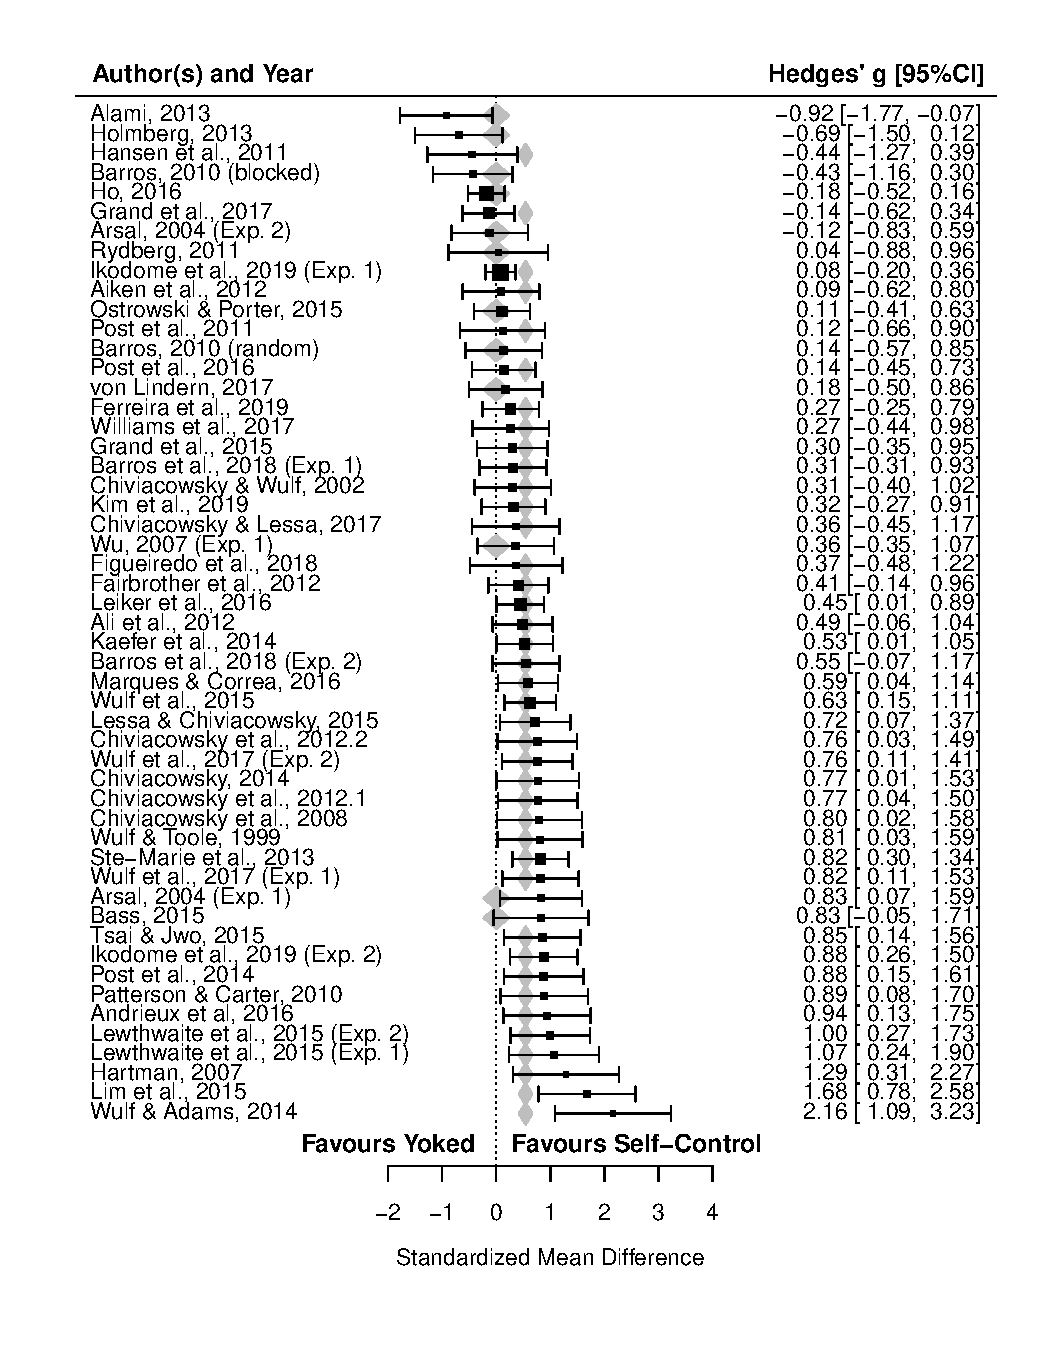
\includegraphics[scale=0.9]{figs/fig2.pdf}
    \label{fig:Figure2}
\end{figure}

\subsection{Selection model}
The weight-function model combines an effect size model and a selection model \parencite{Hedges1996-yh}. The effect size model is equivalent to the naïve random effects model, specifying what the distribution of effect sizes would be in the absence of publication bias or other selection effects. The selection model accounts for the probability a given study survives selection based on its \emph{p}-value and specifies how the effect size distribution is modified by selection. A weight-function model with a \emph{p}-value cutpoint of (one-tailed) .025 was fit to the retention effect size estimates. The results of a likelihood ratio test suggest the adjusted model was a significantly better fit to the data than the unadjusted model, $\chi^2(df = 1) = 21.18, p < .0001$.\footnotemark \,The adjusted effect size estimate was significantly different from zero, $g = .107, p < .001, \,95\%\,CI \,[.05, \,.17]$. According to the adjusted model, non-significant results were 6\% as likely to survive selection as significant results (see Figure~\ref{fig:Figure3}).

\footnotetext{Be aware that the likelihood ratio test is not robust to misspecification of the random effects model \parencite{Hedges1996-yh}}

\subsection{\emph{P}-curve}
The purpose of the \emph{p}-curve analysis was to investigate the evidential value in the published reports (\emph{N} = 26) of statistically significant self-controlled learning benefits. Visual inspection of Figure~\ref{fig:Figure4} reveals a v-shaped distribution with the greatest frequency of \emph{p}-values in the $< .05$ bin. The observed \emph{p}-curve was significantly flatter than would be expected if the experiments had 33\% power, $p = .0035$, indicating an absence of evidential value. Conversely, the half \emph{p}-curve \parencite{Simonsohn2015-mn} was significantly right skewed, suggesting the presence of evidential value. Sensitivity analysis, however, revealed that the half curve does not remain significantly right skewed following removal of the most extreme \emph{p}-value from the sample.

\begin{figure}[h]
	\caption{Funnel plot of self-controlled learning studies at retention. Standard error is plotted on the y-axis and Hedges' g is plotted on the x-axis.  Red line represents naïve random effects model estimate (g = .44); blue line represents weight-function model adjusted estimate (g = .11); black contour lines represent two-tailed p-values of .05. In the absence of bias (and other forms of heterogeneity), the most precise experiments would centre on the naïve random effects estimate near the bottom of the plot and as experiments get progressively less precise they would move up the plot and spread out symmetrically. In the presence of bias, one would expect experiments to track to the right side of the positive contour line. The clustering of experiments just to the right of the positive contour line in the above plot suggests substantial bias.}
	\centering
	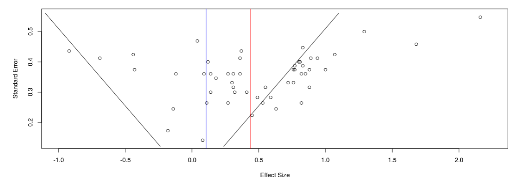
\includegraphics[scale=1.75]{figs/fig3.pdf}
    \label{fig:Figure3}
\end{figure}

\subsection{Interim discussion}
The primary results described above suggest that selection effects have caused a seriously distorted record of self-controlled learning. Estimated benefits are less than one third of the naïve estimate, $g = .107, \,95\%\,CI \,[-.047, \,.18]$. The \emph{p}-curve analysis failed to detect robust evidence of a self-controlled learning effect. The performance of the weight-function model depends on the specific conditions present in the meta-analysis, although these conditions are unknowable \parencite{Carter2019-vv}. It was necessary to conduct sensitivity analyses with additional bias correction methods to assess the reliability of the selection-adjusted weight-function model estimate. Based on performance checks conducted under a range of plausible conditions, it was determined that sensitivity analyses conducted with a PEESE meta-regression and \emph{p}-curve effect size estimation would provide good performance coverage across most plausible conditions.

\vspace{12pt}
\begin{figure}[H]
	\caption{p-curve analysis of published experiments that were statistically significant at retention. If the included experiments are studying a true null hypothesis the expected distribution of p-values is uniform, represented by the dotted line. If the experiments are studying a true effect, the expected distribution becomes increasingly right skewed as a function of statistical power. The expected right skewed distribution associated with 33\% power is plotted by the dashed line. The observed p-curve is plotted by the solid line and was substantially flatter than the 33\% power distribution. The half p-curve analysis included p-values below p = .025 and was significantly right skewed. The right skew did not survive deletion of the most extreme value.}
	\centering
	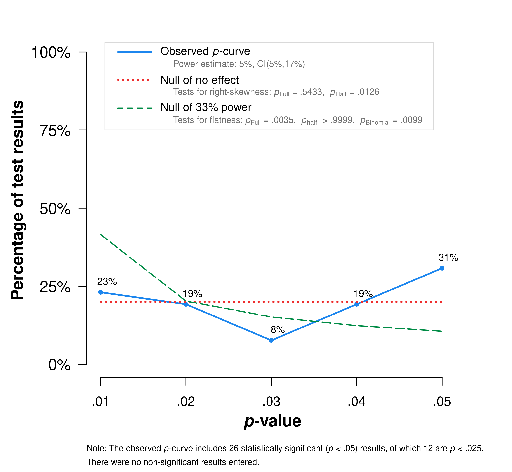
\includegraphics[scale=1.5]{figs/fig4.pdf}
    \label{fig:Figure4}
\end{figure}

\section{Sensitivity analyses} 
\subsection{Precision-effect with standard error (PEESE) model}
When publication bias is present in a body of evidence, sample size and effect size can be negatively correlated \parencite{Stanley2014-xl}. The PEESE model fits a quadratic relationship between effect size and standard error to reflect the intuition that publication bias is stronger for low precision studies than high precision studies. The rationale is that low precision studies need to overestimate effects to achieve significance and get published, while high precision studies can publish without exaggerated effects; thus, creating greater publication bias among lower precision studies \parencite{Carter2019-vv,Stanley2014-xl}. A weighted-least-squares regression model was fit with effect size regressed on the square of the standard error, weighted by the inverse of the variance:
\[g_{i} = b_{0} + b_{1}se_{i}^2 + e_{i}\]
The PEESE method estimated a non-significant benefit of self-controlled learning after controlling for publication bias, $g = .054, p = .659$.

\subsection{\emph{P}-curve effect estimation}
A \emph{p}-curve model was fit to the overall retention effect size data, unlike the first primary \emph{p}-curve which was fit to the reported significant results. The \emph{p}-curve is a function of sample size and effect size, and because sample size is known, the effect size that provides the best fit to the observed \emph{p}-curve can be estimated \parencite{Simonsohn2014-xq}. A \emph{p}-curve analysis conducted with the \texttt{dmetar} package \parencite{Harrer2019-yv} in \texttt{R} was used to estimate the average effect size among the statistically significant effects in the meta-analysis. The model estimated an average effect of $g = .035$.\footnotemark

\footnotetext{The \emph{p}-curve of effect sizes was significantly flatter than the expected 33\% power curve as well, $p = .009$}

\subsection{Acquisition and transfer}
In light of the evidence that experiments are apparently selected for positive self-controlled learning effects at retention, conducting pre-planned exploratory estimates of the effect of self-controlled practice on acquisition and transfer performance was deemed no longer appropriate. The primary take away from the analysis is that the reported self-controlled learning effects to date are unreliable.

\section{Discussion}
The primary objective of this meta-analysis was to assess the effect of providing choices during the acquisition of a motor skill on delayed retention performance in the general population. A secondary objective was to test between motivation and informational explanations for self-controlled learning benefits by investigating whether choice-type moderates the effect of choice. To this aim, an extensive search for experiments that compared self-controlled practice to a yoked comparison group was conducted. Effect size and moderator data were ascertained from data reported in the research articles or, in some cases, received directly from the authors of the studies. Efforts were taken to ensure that each effect size calculation and moderator code could be reproduced by an independent party. In parallel, the results of published experiments that achieved a hypothesized statistically significant result in favour of self-control were extracted directly from the articles and outlined in a \emph{p}-curve disclosure form (see Appendix A). Pre-registered primary analyses were applied to the data and results were followed up with a suite of sensitivity analyses.

The naïve random effects model estimated a benefit from self-controlled practice of $g = .44$. However, the naïve model fails to account for selection effects, such as publication bias and \emph{p}-hacking, and as such overestimates the true average effect when these selection effects are present \parencite{Carter2019-vv,Hedges1996-yh,Stanley2014-xl}. Publication status was a significant moderator of the self-controlled practice effect, accounting for 48\% of the total heterogeneity in the model. Published experiments reported an average benefit of $g = .54$ while unpublished experiments reported no benefit at all on average. It is possible that researchers use statistical significance, typically defined as $p < .05$ on a two-tailed test, to filter their results for publication. To account for potential selection effects driven by statistical significance, a weight-function model was fit to the retention test effect size data with a one-tailed \emph{p}-value cutpoint of .025 included in the model \parencite{Vevea1995-uv}. The adjusted model provided a significantly better fit to the data than the naïve random effects model. The model estimated the selection-adjusted benefit of self-controlled learning as $g = .11$, a dramatic departure from the naïve estimate of $g = .44$. Two additional bias correction techniques were conducted to assess the sensitivity of this result to changes in correction methodology. The PEESE method estimated the effect at $g = .05$, while \emph{p}-curve estimated $g = .04$, and neither analysis was able to rule out the null hypothesis.

In parallel to the meta-analysis described above, a \emph{p}-curve was conducted on the reported significant results. The \emph{p}-curve used somewhat different inclusion criteria focusing only on published, statistically significant results suggesting a self-controlled learning benefit. In addition, the \emph{p}-curve included results reported for any dependent measure in an article, even if the focal measure (of this meta-analysis) was reported as non-significant. Therefore, the \emph{p}-curve was more inclusive of evidence reported by authors as favouring a self-controlled benefit while ignoring experiments with null effects. The results revealed both significant right skew below $p = .025$ (two-tailed) and a \emph{p}-curve that was significantly flatter than a distribution with an expected power of 33\%. The evidence of right skew, indicating superiority of self-control relative to yoked conditions, was tenuous and did not survive the deletion of the most extreme result--an experiment that reported a benefit from self-control of $g =  2.16$ \parencite{Wulf2014-ti}. The overall \emph{p}-curve produced an estimate that the true power of the included experiments was 5\%, leading to a rejection of the hypothesis that the experiments contained evidential value.

It appears from these analyses that the substantial self-controlled learning literature is, as of now, insufficient to provide evidence that self-controlled practice is more effective than a yoked practice. The bias correction techniques applied in this analysis are sensitive to unknown conditions, such as the true average effect size and the amount of true heterogeneity; although efforts were taken to provide coverage across most plausible conditions. The corrected estimates produced by the weight-function model, \emph{p}-curve, and PEESE methods appeared to converge on trivially small effects. Further, the \emph{p}-curve of significant results suggested a lack of evidential value. Based on the model performance parameters we simulated \parencite{Carter2019-vv}, point estimates of the self-controlled learning effect ranging from $g = -.11$ to $.26$ are plausible, with plausible upper confidence limits of $g = .33$. Thus, this analysis does not rule out the possibility that self-controlled practice provides meaningful motor learning benefits on average. The present literature, however, appears insufficient to establish that a self-control benefit indeed exists.

Turning to the current theoretical debates surrounding the motivational and informational underpinnings of self-controlled learning, these debates now seem moot, or at least premature. The effectiveness of self-control was not moderated by choice-type, suggesting that self-controlled practice may be ineffective regardless of the nature of the choices provided. Indeed, the only factor we tested that moderated the effect of self-controlled practice was publication status.

\subsection{Future studies}
Given that the current meta-analysis failed to support the widely touted assertion of a substantial self-controlled learning benefit \parencite{Sanli2013-xn,Ste-Marie2019-bw,Wulf2016-gf}, considerations need to be given to the design and research practices for future studies. Registered reports provide one possible path forward \parencite{Caldwell2020-jg}. A registered report involves submitting a research proposal to a two-phase peer-review. The first phase of the review occurs prior to data-collection and is assessed based on the proposed methodology, rationale, and potential contribution. If accepted in principle, researchers commit to carrying out the registered experiment and submitting the results in a final article for the second phase of peer-review. The final article is peer-reviewed for quality and adherence to the registered plan, but accept-reject decisions at this point are not based on the results. In theory, this practice should eliminate \emph{p}-hacking and, for literatures composed entirely of registered reports, publication bias. A number of motor behaviour and/or kinesiology journals have begun adopting registered reports as an option for authors, including the \emph{Human Movement Science}, \emph{Frontiers in Movement Science and Sport Psychology}, \emph{Journal of Sport and Exercise Psychology}, and \emph{Registered Reports in Kinesiology}.

While registered reports are a potentially fruitful process to begin the accumulation of evidence regarding self-controlled learning, there are practical issues with investigating self-controlled learning that motor learning researchers may find overly burdensome. For example, to have 80\% power to detect an effect of $g = .26$ with a two cell experimental design, 506 participants are required. If the weight-function adjusted estimate of $g = .11$ is accurate, \emph{N} = 2600 are required. More challenging still would be testing between hypothesized motivational and informational mechanisms. For example, if a 2 (choice) X 2 (choice-relevance) experiment were conducted to test whether the instructional-relevance of choice fully attenuates its effect, four times as many participants would be required to maintain the same degree of power \parencite{Simonsohn2014-blog}. In contrast, the median sample size among experiments included in this meta-analysis was \emph{N} = 36, which is typical of motor learning experiments in general \parencite{Lohse2016-cf}.

In addition to challenges with establishing that an effect exists, additional challenges will emerge if researchers are interested in generalizing the benefits of self-controlled practice beyond comparisons to a yoked group, as has been the case thus far \parencite{Ste-Marie2019-bw,Wulf2016-gf}. Yoking may allow for inferences to be made about the act of making certain choices, but it may not provide an adequate control group for evaluating best practices in an applied setting \parencite[e.g.,][]{Barros2019-my,Ste-Marie2019-bw,Yantha2019-dt}. Indeed, given that our estimate suggests the advantage of self-controlled over yoked practice is small, if it exists at all, it seems unlikely that self-control would be more effective than an instructor-guided practice. An instructor-guided group could easily be argued to have advantages over a yoked group, because of the ability for the instructor to adapt choices to the current practice context and to make use of personal experience and expertise. Following this logic, experiments investigating the benefit of self-controlled over instructor-guided practice could conceivably require substantially larger samples than experiments that use yoked comparison groups.

\subsection{Exploratory analysis of pre-registered experiments}
There have been, to our knowledge, four pre-registered experiments that have compared self-controlled and yoked practice \parencite{Grand2017-de,McKay2020-vj,StGermain2020-naspspa,Yantha2019-dt}. Three of these experiments failed to meet our inclusion criteria because they were not published or part of an accepted thesis at the time of the analysis \parencite{McKay2020-vj,StGermain2020-naspspa,Yantha2019-dt}. These pre-registered experiments should provide estimates of the self-control effect unbiased by selection effects and are therefore more useful for estimating the real average effect than attempting to correct biased experiments after the fact \parencite{Carter2019-vv}. A random effects model was used to estimate the average effect of self-control in the four experiments and yielded $g = .02, \,95\%\,CI \,[-.17, \,.21]$. These results converge with the bias-corrected estimates around trivially small differences between self-controlled and yoked practice conditions.

\subsection{Conclusion}
We set out to assess the effect of self-controlled practice on motor learning. The published literature on the subject to date appeared unambiguously supportive of a self-control benefit, yet the results of this meta-analysis suggest this may not be the case. If authors, reviewers, and editors select for statistical significance when deciding if experiments get published, the published literature becomes biased \parencite{Ioannidis2005-km}. Worse still, filtering based on statistical significance may well incentivize researchers to leverage researcher degrees of freedom to achieve a significant result, a practice known as \emph{p}-hacking, further biasing the literature \parencite{Wicherts2016-qz}. An instructive example of the potential impact of selection effects comes from research studying the so-called ego-depletion effect \parencite{Baumeister2007-rb,Hagger2010-cs}. In a typical study, participants are asked to engage in activities that supposedly drain a limited reservoir of willpower, termed ego-depletion, and are subsequently measured on a dependent measure requiring an additional exertion of self-control, such as a Stroop task. The typical finding is that performance suffers on the second task if ego-depletion occurs beforehand. A meta-analysis by Hagger and colleagues (\citeyear{Hagger2010-cs}) reported the average effect of ego-depleting interventions on willpower dependent measures was $d = .62$. There was apparent consensus in the field that willpower relied on a limited resource due to the ostensibly unambiguous evidence in support of the theory \parencite{Baumeister2016-df}. Nevertheless, when bias correction methods were applied in a meta-analysis of ego-depletion literature, the adjusted estimates often did not differ significantly from zero \parencite{Carter2015-zk}. Subsequently, a pre-registered, multi-lab replication project tested a sample of \emph{N} = 2141 and reported that the ego-depletion effect was close to zero \parencite{Hagger2016-ay}. Thus, a prominent psychological construct substantiated by a large corpus of peer-reviewed evidence was investigated using cutting edge meta-analytic techniques that corrected for selection bias and the result was a trivially small estimated effect--an estimate supported by a subsequent large scale pre-registered replication effort. Notably, both the bias corrected meta-analysis and the subsequent multi-lab replication efforts have been criticized by ego-depletion theorists \parencite{Cunningham2016-qy,Baumeister2016-df}. Others have sharply challenged these critiques \parencite[e.g.,][]{Schimmack2020-ea}, and while debate continues among social psychologists about the underlying theory at stake \parencite[e.g.,][]{Dang2018-xa}, there is consensus that several methods shown to produce positive results in the past are unlikely to replicate in future experiments.

In stark parallel to the ego-depletion literature, the findings of the current research suggest the self-controlled motor learning literature may be similarly biased. As motor learning researchers consider the path forward for self-controlled learning, non-bias related limitations of the extant literature should be addressed. For example, yoked groups fail to isolate putative motivational and informational processes when self-controlling learners make choices pertinent to acquiring a skill \parencite{Carter2016-fq,Carter2017-mk,Lewthwaite2015-bd}. Further, exclusive reliance on yoked comparison groups limits the generalizability of self-controlled learning to applied settings where the alternative to self-control is typically coach or instructor control (i.e., those with domain-specific knowledge). As motor learning researchers in this area move forward, they are faced with the question of whether this effect is worth the resources required to study it. If that answer is yes, then in addition to being pre-registered and an adequately powered design, future self-controlled learning experiments should provide insight about either the underlying processes at work or the real world usefulness of this practice variable.

\section{Data and code availability}
All data and code associated with this articile is available at \href{https://osf.io/fhwse/}{https://osf.io/fhwse/}.

\printbibliography

\appendix
\begin{landscape}
\section{\emph{p}-curve disclosure form}
\setstretch{1}
\footnotesize
\begin{longtable}[l]{p{2cm}p{5.5cm}p{3cm}p{2cm}p{6cm}p{1.5cm}}
	\caption{\\ Experiment information from papers included in the p-curve analysis.}
	\label{tab:TableA1}\\
\hline
  \textbf{Original paper} &
  \textbf{Quoted text from original paper indicated predicted benefit of self-control relative to yoked practice} &
  \textbf{Design} &
  \textbf{Key statistical  result} &
  \textbf{Quoted text from original paper with statistical result} &
  \textbf{Result}
  %\textbf{Robustness result} 
  \\
\hline
\endfirsthead
%
\hline
  \textbf{Original paper} &
  \textbf{Quoted text from original paper indicated predicted benefit of self-control relative to yoked practice} &
  \textbf{Design} &
  \textbf{Key statistical  result} &
  \textbf{Quoted text from original paper with statistical result} &
  \textbf{Result}
  %\textbf{Robustness result} 
  \\
\hline
\endhead
%
Andrieux, Danna \& Thon (2012) &
  ``Thus, we hypothesized that a practice condition in which the learner could set the level of task difficulty would be more beneficial for learning than a condition in which this parameter was imposed.'' &
  Two cell &
  Difference in means &
  ``A follow up analysis restricted to the first two blocks revealed a significant difference between groups, $F(1, 36) = 4.85, p < .05, \eta_{p}^2 = .12$. Self-controlled learners were significantly more accurate (M AE = 12.73 mm, SE = 1.57) than their yoked counterparts (M AE = 18.1 mm, SE = 1.87) after a 24-hr rest.'' &
  $F(1, 36) = 4.85$
   \\[3.75cm]
Andrieux., Boutin, \& Thon (2016) &
  ``Two main reasons led us to expect that self-control of nominal task difficulty would enhance motor skill learning, and especially when introduced during early practice rather than during late practice.'' &
  Four cell (Full self-control, full yoked, self-control then yoked, yoked then self-control) &
  Difference in means &
  ``Planned pairwise comparisons revealed that the self-control groups exhibited lower RMSE (SC + SC, SC + YO, and YO + SC groups) than their yoked group counterparts (YO + YO group), $F(1, 44) = 14.02, p < .01$.'' &
  $F(1, 44) = 14.02$
   \\[2.5cm]
Brydges, Carnahan, Safir \& Dubrowski (2009) &
  ``We hypothesised that participants with self-guided access to instruction would learn more than participants whose access to instruction was externally controlled.'' &
  2 (Control: self, yoked) X 2 (Goals: process, outcome) &
  Difference in means &
  ``The self-process group performed better on the retention test than the control-process group (Fig. 1). This effect was significant for time taken, ($F[1,23] = 4.33, P < 0.05$).'' &
  $F(1,23) = 4.33$
   \\[3cm]
Chiviacowsky (2014) &
  ``We hypothesized that participants of the self-controlled group would show superior motor learning than yoked participants'' &
  Two cell &
  Difference in means &
  ``The Self group outperformed the Yoked group. The group main effect was significant, $t(26) = 2.08, p = .04, d = .78$.'' &
  $t(26) = 2.08$
   \\[1.75cm]
Chiviacowsky, Wulf, de Medeiros, Kaefer \& Tani (2008) &
  ``Therefore, the purpose of the present study was to examine whether the learning benefits of self-controlled KR would generalize to children.'' &
  Two cell &
  Difference in means &
  ``The self-control group had higher accuracy scores than the yoked group. This difference was significant, $F(1, 24) = 4.40, p < .05$.'' &
  $F(1, 24) = 4.40$ 
   \\[2.25cm]
Chiviacowsky, Wulf, Lewthwaite, \& Campos  (2012) &
  ``The potential benefits of self-controlled practice have yet to be examined in persons with PD...under the assumption that self-controlled practice would enhance the learning of the task...'' &
  Two cell &
  Difference in means &
 ``The self-control group was overall more effective than the yoked group. Time in balance was significantly longer for the self-control group, $F(1, 26) = 4.25, p < .05$''. &
  $F(1, 26) = 4.25$
   \\[2.75cm]
Chiviacowsky Wulf, Machado \& Rydberg (2012) &
  ``We predicted that self-controlled practice, in particular the ability to choose when to receive feedback, would result in more effective learning compared to a practice condition without this opportunity (yoked group).'' &
  Two cell &
  Difference in means &
  ``The day following practice, a retention test (without feedback) revealed lower AEs for the self-control group than the yoked group (see Figure 2, right). The group difference was significant, with $F(1, 28)= 4.72, p < 0.05, \eta^2=.14$.'' &
  $F(1, 28)= 4.72$
   \\[3cm]
Hartman (2007) &
  ``The primary aim of this study was to test whether there would exist a learning advantage for a self-controlled group, as opposed to a yoked control group, for learning a dynamic balance task.'' &
  Two cell &
  Difference in means &
  ``To assess the relatively permanent or learning effects of practice with or without a self-controlled use of a balance pole, both groups performed a retention test on Day 3. The group effect was significant, $F(1, 17)  = 8.29, p < .01$, with the Self-control group outperforming the yoked group.'' &
  $F(1, 17) = 8.29$
   \\
Kaefer, Chiviacowsky, Meira Jr. \& Tani (2014) &
  ``...both self-controlled groups (introverts and extroverts) will achieve a level of activation that facilitates learning through the control of stimulation source (feedback) in comparison with the groups that do not have control over it.'' &
  2 (Control: self, yoked) X 2 (Personality: introvert, extrovert) &
  Difference in means &
  ``The groups’ main effects were detected on the factor ``feedback type'': Self-controlled groups performed better, $F(1, 52) = 4.13, p < .05$, compared with externally controlled groups'' &
  $F(1, 52) = 4.13$
   \\[3cm]
Leiker, Bruzi, Miller, Nelson, Wegman \& Lohse (2016) &
  ``We hypothesized that participants in the self-controlled group would show superior learning (i.e., better performance on retention and transfer tests) compared to the yoked group.'' &
  Two cell &
  Difference in means &
  ``Controlling for pre-pest, there was a significant main effect of group, $F(1,57) = 4.51, p = 0.04, \eta_{p}^2 = 0.07$, such that participants in the self-controlled group performed better on the post-test than participants in the yoked group.'' &
  $F(1,57) = 4.51$
   \\[3cm]
Lemos, Wulf, Lewthwaite \& Chiviacowsky (2017) &
  ``Independent of which factor the learner is given control over e or whether or not this factor is directly related to the task to be learned e the learning benefits appear to be very robust.'' &
  Two cell &
  Difference in means &
  ``On the retention test, choice participants clearly outperformed the control group. The group main effect was significant, $F(1, 22) = 88.16, p < 0.01$.'' &
  $F(1, 22) = 88.16$
   \\[2.5cm]
Lessa \& Chiviacowsky (2015) &
  ``...it was hypothesized that older adult participants of the self-group would demonstrate superior motor learning results, presenting faster task times on the speed cup-stacking task, when compared with participants in the yoked control group.'' &
  Two cell &
  Difference in means &
  ``The analysis of the retention test revealed significant differences between groups, $F(1,34) = 4.87, p < .05$...with participants of the self-control group presenting faster task times compared to yoked participants.'' &
  $F(1,34) = 4.87$
   \\
Lewthwaite, Chiviacowsky, Drews \& Wulf (2015; Exp. 1) &
  ``In the present experiment, the choice learners were given was not related to task performance per se. Therefore, any learning benefits resulting from having, as opposed to not having, a choice would suggest that motivational factors are responsible for those effects.'' &
  Two cell &
  Difference in means &
  ``On the retention test, during which white golf balls were used, the choice group showed significantly higher putting accuracy (36.8) than the yoked group (26.4), $F(1, 22) = 7.31, p < .05$'' &
  $F(1, 22) = 7.31$
   \\[3.5cm]
Lewthwaite, Chiviacowsky, Drews \& Wulf (2015; Exp. 2) &
  ``Given the potential theoretical importance of the finding in Experiment 1, we wanted to replicate it with another task and different type of choice.'' &
  Two cell &
  Difference in means &
  ``On the retention test 1 day later, the choice group demonstrated significantly longer times in balance than the yoked group, $F(1, 27) = 7.93, p < .01$.'' &
 $F(1, 27) = 7.93$
   \\[2.5cm]
Lim, Ali, Kim, Choi \& Radlo (2015) &
  ``It was expected that a self-controlled feedback schedule would be more effective for the learning and performance of serial skills for both acquisition and retention phases than a yoked schedule.'' &
  Two cell &
  Difference in means &
  ``In the retention phase, there was a significant main effect for Group ($F(1, 22) = 18.27, p < .05$). The follow-up test indicated that the Self-controlled feedback group had higher performance (Cohen's $d = 6.4$) than the Yoked-feedback group during the retention test in both blocks.'' &
  $F(1, 22) = 18.27$
   \\[3.5cm]
Patterson, Carter \& Sanli (2011: comparison 1) &
  ``We expected that the structure of this self-controlled practice context would either add to or compromise the existing benefits attributed to a self-controlled practice context.'' &
  2 (Control: self, yoked) X 3 (Structure: full, all, faded) &
  Difference in means &
  ``Specifically, the Self-Self condition demonstrated less |CE| compared to their Yoked-Yoked counterparts. This main effect was significant, $F(1, 18) = 8.06, p < .05$.'' &
  $F(1, 18) = 8.06$
   \\[3.5cm]
Patterson, Carter \& Sanli (2011: comparison 2) &
  ``We expected that the structure of this self-controlled practice context would either add to or compromise the existing benefits attributed to a self-controlled practice context.'' &
  2 (Control: self, yoked) X 3 (Structure: full, all, faded) &
  Difference in means &
  ``The All-Self condition demonstrated less |CE| compared to the All-Yoked condition. This main effect was also statistically significant, $F(1, 18) = 4.67, p < .05$.'' &
  $F(1, 18) = 4.67$
   \\[2.25cm]
Patterson, Carter \& Sanli (2011: comparison 3) &
  ``We expected that the structure of this self-controlled practice context would either add to or compromise the existing benefits attributed to a self-controlled practice context.'' &
  2 (Control: self, yoked) X 3 (Structure: full, all, faded) &
  Difference in means &
  ``The Faded-Self condition demonstrated less |CE| compared to the Faded-Yoked condition, supported by a main effect for group, $F(1, 18) = 5.78, p < .05$.'' &
  $F(1, 18) = 5.78$
   \\[2.25cm]
%Patterson, Carter \& Hansen (2013) &
%  ``We predicted the following: participants self-controlling their KR schedule would demonstrate superior learning compared to those who do not engage in the increased processing demands used to individualize their KR schedule.'' &
%  2(KR Condition: self, yoked) X 2 (Schedule: random, blocked) &
%  Difference in means &
%  ``The analysis revealed main effects of KR Condition, $F(1,40) = 4.40, p < .05$.'' &
%  $F(1,40) = 4.40$
%   \\[3cm]
Post, Fairbrother, Barros \& Kulpa (2014) &
  ``It was hypothesized that learners in the SC group would demonstrate superior accuracy and form scores compared with the yoked group during the retention test.'' &
  Two cell &
  Difference in means &
  ``The univariate ANOVA for retention revealed a significant group effect, $F(1, 29) = 6.08, p = .020$. The SC group had higher Accuracy scores the YK group'' &
  $F(1, 29) = 6.08$
   \\[2.25cm]
Ste-Marie, Vertes, Law \& Rymal (2013) &
  ``We hypothesized that the Learner Controlled group would show superior physical performance of the trampoline skills… compared to the Experimenter Controlled group.'' &
  Two cell &
  Difference in means &
  ``A separate independent samples t-test showed that the Learner Controlled group had significantly higher performance scores compared to the Experimenter Controlled group at retention, $t(58) = 3.21, p < .05, d = .753$.'' &
  $t(58) = 3.21$
   \\
Wulf \& Adams (2014) &
  ``We asked whether giving performers an incidental choice would also result in more effective learning of exercise routines.'' &
  2(Group: self-control, yoked) X 3 (Exercise: toe touch, head turn, ball pass) X 2 (Leg: left, right) mixed design with repeated measures on the final two factors &
  Difference in means &
  ``On the retention test… the choice group showed fewer errors than the control group. The main effects of group, $F(1,18) = 25.35, p < .001$, was significant.'' &
  $F(1,18) = 25.35$
   \\[4.5cm]
Wulf \& Toole (1999) &
  ``If the beneficial effects of self-control found in previous studies are more general in nature (i.e., some general mechanism responsible for these effects), learning advantage would also be expected for self-controlled use of physical assistance.'' &
  Two cell &
  Difference in means &
  ``The main effect of Group, $F(1,24) = 4.54, p < .05$, was significant. Thus, allowing learners to select their own schedule of physical assistance during practice had a clearly beneficial effect on learning.'' &
  $F(1,24) = 4.54$
   \\[3.5cm]
Wulf, Clauss, Shea \& Whitacre (2001) &
  ``Importantly, however, if self-control promotes the development of a more efficient movement technique, one should see greater movement efficiency, as indicated by delayed force onsets, in self-control as compared to yoked participants.'' &
  Two cell &
  Difference in means &
  ``Whereas the self-control group demonstrated relative force onsets that, on average, occurred about half the distance between the center of the apparatus and the participant's maximum amplitude, the yoked group’s average force onset had already occurred after they had travelled less than 20\% of the distance to the maximum amplitude. This group difference was significant, $F(1,24) = 4.43, p < .05$.'' &
 $F(1,24) = 4.43$
   \\
Wulf, Raupach \& Pfeiffer (2005) &
  ``Thus, if the learning advantages of self-controlled practice generalize to observational practice, allowing learners to decide when they want to view a model presentation should result in enhanced retention performance, with regard to movement form and, perhaps, movement accuracy, compared to that of yoked learners.'' &
  Two cell &
  Difference in means &
  ``Overall, the self-control group had higher form scores than the yoked group throughout retention. The main effect of group $F(1,23) = 5.16, p < .05$, was significant.'' &
  $F(1,23) = 5.16$
   \\[4.5cm]
Wulf, Iwatsuki, Machin, Kellogg, Copeland, \& Lewthwaite (2017) Exp 1. &
  ``The purpose of the present experiments was threefold. First, we deemed it important to provide further evidence for the impact of incidental choices on motor skill learning. Given that self-controlled practice benefits for learning have frequently been interpreted from an information-processing perspective (e.g., Carter, Carlson, \& Ste-Marie, 2014; Carter \& Ste-Marie, 2016), with limited regard for rewarding-motivational explanations, further experimental evidence for learning enhancements through choices not directly related to the task seemed desirable (Experiments 1 and 2).'' &
  Two cell &
  Difference in means &
  ``On the retention test one day later, the choice group demonstrated higher scores than did the control group. The group effect was significant, $F(1, 29) = 5.72, p < .05$.'' &
  $F(1, 29) = 5.72$
   \\
Wulf, Chiviacowsky \& Drews (2015) &
  ``To summarize, we hypothesized that an external focus and autonomy support would have additive benefits for motor learning (i.e., retention and transfer performance), as evidenced by main effects for each factor.'' &
  2 (Autonomy support: self, yoked) X 2 (Focus: external, internal) &
  Difference in means &
  ``On the retention test, the main effect of Autonomy Support was significant, $F(1, 64) = 6.98, p < .01$.'' &
  $F(1,64) = 6.98$
   \\[3.25cm]
Ikudome, Kuo, Ogasa, Mori \& Nakamoto (2019; Exp. 2) &
  ``Previous studies manipulating participants’ choice of variables relevant to the experimental task have indicated that such choices have a positive effect on motor learning due to deeper information processing by the participants. Based on these studies, it is possible that this positive effect would be observed regardless of participants’ levels of intrinsic motivation, because this type of choice would not induce a change in perceived locus of causality from internal to external.'' &
  2(Choice: self, yoked) X 2 (Motivation: high, low) &
  Difference in means &
  ``An ANCOVA indicated significant main effects of choice, $F(1, 39) = 8.93, p = .005$.'' &
  $F(1,39) = 8.93$
	\\
\hline
\end{longtable}
\end{landscape}

\end{document}

%%
%% Copyright (C) 2019 by Daniel A. Weiss <daniel.weiss.led at gmail.com>
%%
%% This work may be distributed and/or modified under the
%% conditions of the LaTeX Project Public License (LPPL), either
%% version 1.3c of this license or (at your option) any later
%% version.  The latest version of this license is in the file:
%%
%% http://www.latex-project.org/lppl.txt
%%
%% Users may freely modify these files without permission, as long as the
%% copyright line and this statement are maintained intact.
%%
%% This work is not endorsed by, affiliated with, or probably even known
%% by, the American Psychological Association.
%%
%% This work is "maintained" (as per LPPL maintenance status) by
%% Daniel A. Weiss.
%%
%% This work consists of the file  apa7.dtx
%% and the derived files           apa7.ins,
%%                                 apa7.cls,
%%                                 apa7.pdf,
%%                                 README,
%%                                 APA7american.txt,
%%                                 APA7british.txt,
%%                                 APA7dutch.txt,
%%                                 APA7english.txt,
%%                                 APA7german.txt,
%%                                 APA7ngerman.txt,
%%                                 APA7greek.txt,
%%                                 APA7czech.txt,
%%                                 APA7turkish.txt,
%%                                 APA7endfloat.cfg,
%%                                 Figure1.pdf,
%%                                 shortsample.tex,
%%                                 longsample.tex, and
%%                                 bibliography.bib.
%%
%%
%% End of file `./samples/longsample.tex'.
